\documentclass[12pt]{report}

\usepackage{../1_CasesDB/Common/articlePreamble}



\begin{document}

% titlepage

\begin{titlepage}
    \begin{center}
        \vspace*{1in}
        \Huge
        \textbf{Case Report}


        \vspace{0.5in}
        \LARGE
        \textbf{Optometry Case Studies}\\
        
        \textbf{An Exploration of Eye Health}
            
        \vspace{0.7in}
        \LARGE
        \textbf{BY}
            
        \vspace{0.7in}
            
        \textbf{Musoke Ntaate Augustine\\}
        % PhD, M.Optom, OD, FAAO}
            
        \vspace{1.2in}
        \LARGE
        % \textbf{A THESIS* SUBMITTED TO THE
        % DIRECTORATE OF RESEARCH AND GRADUATE TRAINING
        % FOR THE AWARD OF THE DEGREE OF DOCTOR OF
        % PHILOSOPHY OF MAKERERE UNIVERSITY}
        
            
        \vspace{0.3in}
        % \vfill
            
        % \includegraphics[width=0.5\textwidth]{figures/logo.jpeg}

        % \vspace{0.5cm}
        % \vfill
        
        \Large
        % Dr Dralega Anguyo, \\
        \today
            
        \vspace{1.1in}

    \end{center}
\end{titlepage}
    


\clearpage
\pagenumbering{roman}


\cleardoublepage
\printglossary[title=Operational Definitions] % Prints glossary without modifying TOC
\pagebreak


\cleardoublepage
\printglossary[type=\acronymtype, title=Abbreviations] % Prints glossary with title "Abbreviations"
\pagebreak



\pagebreak
\tableofcontents

% =======================================================================
\clearpage
\pagenumbering{arabic}

\section{Introduction}

\begin{frame}{Introduction}
    
\begin{itemize}
    \item \parencite{dass2012ocular} and \parencite{almahmoud2019epidemiology} suggested that.
    \item One or two paragraphs summarizing why this case is unique (may include references)
\end{itemize}

\end{frame}


\section{Patient Information}

\begin{itemize}
    \item De-identified patient specific information.
    \item Primary concerns and symptoms of the patient
    \item Medical, family, and psycho-social history including relevant genetic information Reported on Line
    \item Relevant past interventions with outcomes

\end{itemize}


\section{Clinical Findings}

\begin{itemize}
    \item Describe significant physical examination (PE) and important clinical findings
\end{itemize}


\section{Timeline}
\begin{itemize}
    \item Historical and current information from this episode of care organized as a timeline

\end{itemize} 



\section{Diagnostic Assessment}

\begin{itemize}
    \item Diagnostic testing (such as PE, laboratory testing, imaging, surveys)

    \item Diagnostic challenges (such as access to testing, financial, or cultural)

    \item Diagnosis (including other diagnoses considered)

    \item Prognosis (such as staging in oncology) where applicable

\end{itemize}


\begin{table}[htbp]
    \centering
    \caption{Eye Test Results}
    \resizebox{.8\textwidth}{!}{%
        \begin{tabular}{|c|c|c|c|}
            \hline
                \textbf{Date} & \textbf{Visual Acuity} & \textbf{Intraocular Pressure} & \textbf{Remarks} \\ \hline
                2022-01-01 & 20/20 & 15 mmHg & Normal \\ 
                2022-04-15 & 20/25 & 16 mmHg & Slight decrease in visual acuity \\ 
                2022-08-20 & 20/30 & 18 mmHg & Further decrease in visual acuity \\ 
                2023-01-10 & 20/40 & 20 mmHg & Significant decrease in visual acuity \\ 
            \hline
        \end{tabular}%
    }
    

\end{table}
    


\begin{table}[htbp]
    \centering
    \caption{Eye Examination Results for Patient X}
    \label{tab:eye_exam_results}
    \resizebox{.8\textwidth}{!}{%

    \begin{tabular}{ll}
        \toprule
        \textbf{Test} & \textbf{Result} \\
        \midrule
        Visual Acuity (VA) & 20/20 \\
        Refraction Powers & -1.00 (-0.50 @ 180) \\
        Intraocular Pressures (IOP) & 15 mmHg (OD), 16 mmHg (OS) \\
        Pupillary Distance (PD) & 62 mm \\
        Slit Lamp Exam & Normal anterior segment \\
        % Add more rows for additional tests
        Gonioscopy & Open angles \\
        Fundoscopy & Clear optic disc, healthy retina \\
        Visual Fields & Full, no defects \\
        Corneal Topography & Regular astigmatism \\
        \bottomrule
    \end{tabular}

    }
\end{table}


\begin{figure}[htbp]
    \centering
    \resizebox{.6\textwidth}{!}{%
        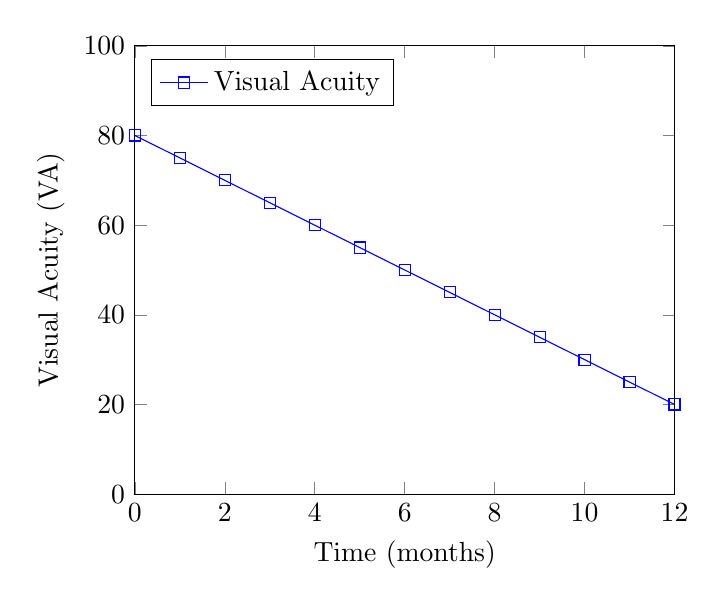
\begin{tikzpicture}
            \begin{axis}[
                xlabel={Time (months)},
                ylabel={Visual Acuity (VA)},
                xmin=0, xmax=12,
                ymin=0, ymax=100,
                xtick={0,2,4,6,8,10,12},
                ytick={0,20,40,60,80,100},
                legend pos=north west,
                grid style=dashed,
            ]
            
            \addplot[
                color=blue,
                mark=square,
            ]
            coordinates {
                (0,80)(1,75)(2,70)(3,65)(4,60)(5,55)(6,50)(7,45)(8,40)(9,35)(10,30)(11,25)(12,20)
            };
            
            \legend{Visual Acuity}
            
            \end{axis}
        \end{tikzpicture}
    }
    \caption{Visual Acuity Over Time}
    \label{fig:va_graph}
\end{figure}



\section{Therapeutic Intervention}


\begin{frame}{Therapeutic Intervention}
    \begin{itemize}
        \item Types of therapeutic intervention (such as pharmacologic, surgical, preventive, self-care)
        \item Administration of therapeutic intervention (such as dosage, strength, duration)
        \item Changes in therapeutic intervention (with rationale)
    \end{itemize}
    
    
    \gls{myopia}, \gls{hyperopia}, \gls{astigmatism} and \gls{presbyopia}
    
    \gls{amblyopia}, \gls{LogMAR E chart} 
    
    \gls{moh}, \gls{who} and \gls{irb}
\end{frame}


\section{Follow-up and Outcomes}
\begin{frame}{Follow-up and Outcomes}
    \begin{itemize}
        \item Clinician and patient-assessed outcomes (if available)
        \item Important follow-up diagnostic and other test results
        \item Intervention adherence and tolerability (How was this assessed?)
        \item Adverse and unanticipated events
    
    \end{itemize}
\end{frame}


\section{Discussion}
\begin{itemize}
\item A scientific discussion of the strengths AND limitations associated with this case report
\item Discussion of the relevant medical literature with references
\item The scientific rationale for any conclusions (including assessment of possible causes)
\item The primary "take-away" lessons of this case report (without references) in a one paragraph conclusion


\end{itemize}



\section{Patients Perspective}
\begin{itemize}
    \item The patient should share their perspective in one to two paragraphs on the treatment(s) they received.
    
\end{itemize}

\section{Informed Consent}
\begin{itemize}
    \item Did the patient give informed consent? Please provide if requested.


\end{itemize}



\pagebreak
\cleardoublepage
\addcontentsline{toc}{section}{References}
\printbibliography

\cleardoublepage



\end{document}





